
\documentclass[a4paper]{article}

%% Language and font encodings
\usepackage[english]{babel}
\usepackage[utf8x]{inputenc}
\usepackage[T1]{fontenc}

%% Sets page size and margins
\usepackage[a4paper,top=2cm,bottom=2cm,left=2cm,right=2cm,marginparwidth=1.75cm]{geometry}

%% Sets row spaces
\usepackage{setspace}
\renewcommand{\baselinestretch}{1.0}

%% packages for tables
\usepackage{booktabs}

%% for hyper links
\usepackage{hyperref}
\hypersetup{hidelinks,
	colorlinks=true,
	allcolors=black,
	linkcolor=blue,
	filecolor=blue,
    urlcolor=blue,
    citecolor=cyan,
	pdfstartview=Fit,
	breaklinks=true}

%% packages for codes
\usepackage{listings}
\usepackage{xcolor}
% \lstset{
%     numbers=left, 
%     numberstyle= \tiny, 
%     keywordstyle= \color{ blue!70},
%     commentstyle= \color{red!50!green!50!blue!50}, 
%     % frame=shadowbox, % 阴影效果
%     rulesepcolor= \color{ red!20!green!20!blue!20} ,
%     % escapeinside=``, % 英文分号中可写入中文
%     xleftmargin=2em,xrightmargin=2em, aboveskip=1em,
%     framexleftmargin=2em
% } 
\lstset{
    basicstyle          =   \sffamily,          % 基本代码风格
    keywordstyle        =   \bfseries,          % 关键字风格
    commentstyle        =   \rmfamily\itshape,  % 注释的风格,斜体
    stringstyle         =   \ttfamily,  % 字符串风格
    flexiblecolumns,                % 别问为什么,加上这个
    numbers             =   left,   % 行号的位置在左边
    showspaces          =   false,  % 是否显示空格,显示了有点乱,所以不现实了
    %numberstyle         =   \zihao{-5}\ttfamily,    % 行号的样式,小五号,tt等宽字体
    showstringspaces    =   false,
    captionpos          =   t,      % 这段代码的名字所呈现的位置,t指的是top上面
    % frame               =   lrtb,   % 显示边框
}

\lstdefinestyle{Python}{
    language        =   Python, % 语言选Python
    %basicstyle      =   \zihao{-5}\ttfamily,
    %numberstyle     =   \zihao{-5}\ttfamily,
    keywordstyle    =   \color{blue},
    keywordstyle    =   [2] \color{teal},
    stringstyle     =   \color{magenta},
    commentstyle    =   \color{red}\ttfamily,
    breaklines      =   true,   % 自动换行,建议不要写太长的行
    columns         =   fixed,  % 如果不加这一句,字间距就不固定,很丑,必须加
    basewidth       =   0.5em,
}

%% packages for appendix
\usepackage[toc,page]{appendix}

%% Useful packages
\usepackage{amsmath}
\usepackage{graphicx}
\usepackage[colorinlistoftodos]{todonotes}
\usepackage[colorlinks=true, allcolors=blue]{hyperref}
\usepackage[numbers,sort&compress]{natbib} 
\usepackage{float}	% used for fix the location of tables and graphics
\usepackage{subfigure}  % multi-pictures in the same line
\newcommand{\upcite}[1]{\textsuperscript{\cite{#1}}}
\newcommand{\topcaption}{%
	\setlength{\abovecaptionskip}{0pt}%
	\setlength{\belowcaptionskip}{10pt}%
	\caption}

%_____________________________________________

\title{\textbf{Numerical Methods Solving ODE}}
\author{
	Ye, Fengyang (3180111549) \\
	Tang, Yuan (3180111524)   \\
	Du, Yiqing (3180112696)   \\
	Shu, Yue (3180111518)     \\
	Li, Ruiqi (3180111638)
}

\begin{document}

    \maketitle

    \section{Introduction}
    
    %_____________________________________________
    At present, Ordinary Differential Equation (ODE) has been widely used in many aspects such as physics, biology and economics. In practical problems, it is particularly important to find the solution of ordinary differential equations. Despite the analytical solution can find the accurate answer, in some practical problems either it is hard to find the analytic solutions or the solving process is too complicated. In this case, it is extremely important to find the numerical solution of ODE by some methods (such as the Euler method, the Runge-Kutta method and the Adams method). 
    
    In this report, we are required to determine the solutions and domains of two initial value problems (IVPs) by using a combination of numerical and analytical methods. 
    
    For problem 1, we are supposed to compute the solution of such a first-order nonlinear IVP: 
	
	\begin{equation} \label{eq:ode1}
	    y' = y^2 + ty + t^2,\quad y(0) = 1 \\ \tag{IVP1}
	\end{equation}
	
	For problem 2, we are supposed to compute the solution of another first-order nonlinear IVP: 
	
	\begin{equation} \label{eq:ode2}
	    y' = y^3 + ty^2 + t^2y + t^3,\quad y(0) = 1 \\ \tag{IVP2}
	\end{equation}
	
	Several numerical methods -- the Euler method, the Runge-Kutta method and the Adams method—have been compared in the process of solving the two practical problems.
	
    \section{Methods}
    Before using numerical methods to calculate, we try to use analytical methods to calculate the accurate answer. The process of the analytical approach is attached to the Appendix \autoref{apdx:power_series}, and the code of numerical methods is in Appendix \autoref{apdx:code}.
	%_____________________________________________
    %analytical
    \subsection{The Euler Method}
	
	The Euler method approximates the value of $\Phi(t)$ in the region $[t_n, t_{n+1}]$ of the curve by a straight line. In this report we mainly talk about four methods—the forward Euler method, the backward Euler method, the trapezium Euler method and the improved Euler method.
	
	The forward Euler method approximate the original curve with a tangent line of slope $f(t_n, y_n)$. The formula is in the form:
	
	\begin{equation}\label{eq.1}
		y_{n+1} = y_n + hf(t_n, y_n), \enspace n = 0,1,2,...
	\end{equation}
	
	The backward Euler method approximate the original curve with a tangent line of slope $f(t_{n+1}, y_{n+1})$. The formula is in the form:
	
	\begin{equation}\label{eq.2}
		y_{n+1} = y_n + hf(t_{n+1}, y_{n+1}), \enspace n = 0,1,2,...
	\end{equation}	
	
	The trapezium Euler method approximate the original curve with a tangent line of slope ${1 \over 2}(f(t_n)+f(t_{n+1}))$. The formula is in the form:
	
		\begin{equation}\label{eq.1}
		y_{n+1} = y_n + {h\over2}(f(t_n, y_n)+f(t_{n+1}, y_{n+1})), \enspace n = 0,1,2,...
	\end{equation}
	
	The improved Euler method combines the forward Euler method and the trapezium Euler method. The formula is in the form:
	
	\begin{equation}\label{eq.3}
		y_{n+1} = y_n + {h \over 2}(f_n + f(t_n + h, y_n + hf(t_n, y_n))), \enspace, n = 0,1,2,...
	\end{equation}	
	
	
	%____________________________________________
	\subsection{The Runge-Kutta Method}
	
	The Runge-Kutta Method is similar to the Euler method, however, in this method, we try to find the slope with a few more points on the region $[t_n, t_{n+1}]$, then taking a weighted average of the slope values at these points, and using the resulting value as the approximate slope $k$.
	In this report we discuss the third-order three-stage Runge-Kutta method and the fourth-order four-stage Runge-Kutta method. The formula of the third-order three-stage Runge-Kutta method is in the form:
	
	\begin{equation}\label{eq.4}
		y_{n+1} = y_n + h(\frac{k_{n1} + 4k_{n2} + k_{n3} }{6}), \enspace n = 0, 1, 2,...
	\end{equation}

	Where
	
	\begin{align} \nonumber
		k_{n1} &= f(t_n, y_n), \\ \nonumber
		k_{n2} &= f(t_n + {1 \over 2}h, y_n + {1 \over 2}hk_{n1}), \\ \nonumber
		k_{n3} &= f(t_n + h, y_n - hk_{n1} + {1 \over 2}hk_{n2}), \\ \nonumber
	\end{align}
	
	The formula of the fourth-order four-stage Runge-Kutta method is in the form:
	
		\begin{equation}\label{eq.4}
		y_{n+1} = y_n + h(\frac{k_{n1} + 2k_{n2} + 2k_{n3} + k_{n4} }{6}), \enspace n = 0, 1, 2,...
	\end{equation}

	Where
	
	\begin{align} \nonumber
		k_{n1} &= f(t_n, y_n), \\ \nonumber
		k_{n2} &= f(t_n + {1 \over 2}h, y_n + {1 \over 2}hk_{n1}), \\ \nonumber
		k_{n3} &= f(t_n + {1 \over 2}h, y_n + {1 \over 2}hk_{n2}), \\ \nonumber
		k_{n4} &= f(t_n + h, y_n + hk_{n3}), \\ \nonumber
	\end{align}
	%_______________________________________
	\subsection{The Adams Method}
	
	The Adams method makes use of a polynomial $P_k(t)$ of degree $k$ to approximate $\Phi'(t)$ and evaluates the integral of $\Phi'(t)$.
	The Second-order Adams-Bashforth formula is
	
	\begin{equation}\label{eq.6}
		y_{n+1} = y_n + {3 \over 2}hf_n - {1 \over 2}f_{n-1}, \  n = 0,1,2,...
	\end{equation}
	
	The Fourth-order Adams-Bashforth formula is
	
	\begin{equation}\label{eq.7}
		y_{n+1} = y_n + {h \over 24}(55f_n - 59f_{n-1} + 37f_{n-2} - 9f_{n-3}), \  n = 0,1,2,...
	\end{equation}
	
	The Adams-Moulton formula is
	
	\begin{equation}\label{eq.7}
		y_{n+1} = y_n + {h \over 24}(9f_{n+1} + 19f_{n} - 5f_{n-1} + f_{n-2}), \  n = 0,1,2,...
	\end{equation}
	%_____________________________________________________
    \subsection{Solutions}
    We define the result computed by ODE113() function in MatLab with a stepsize $h=0.00001$ as the accurate solution. The solutions graph of problem 1 and problem 2 are shown below as \autoref{fig:ivp_sol}.
    
	\begin{figure}[H]
    \centering
    \subfigure[Problem 1]{
    \begin{minipage}{8cm}
        \centering
        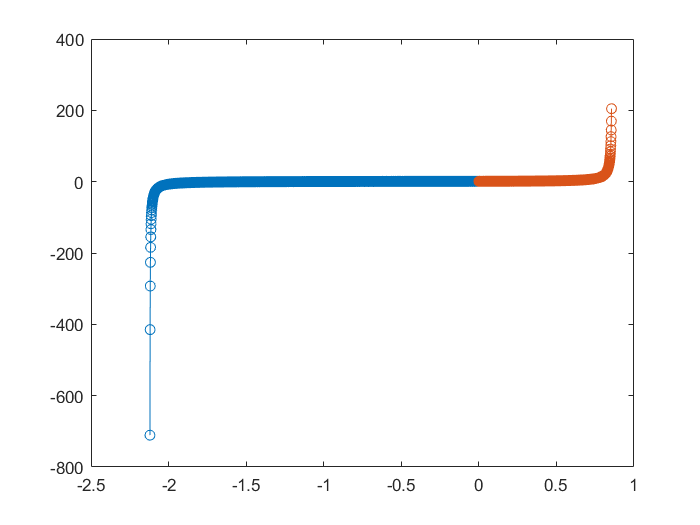
\includegraphics[width=7.5cm]{img/newivp1.png}
    %\caption{fig1}
    \end{minipage}%
    }%
    \subfigure[Problem 2]{
    \begin{minipage}{8cm}
        \centering
        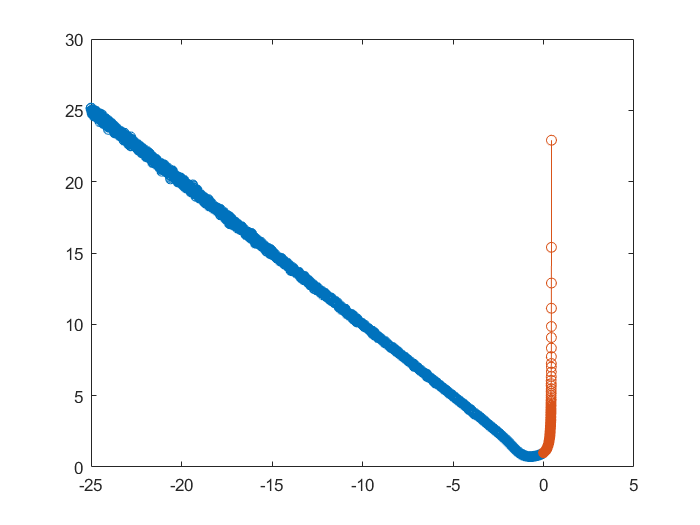
\includegraphics[width=7.5cm]{img/newivp2.png}
    %\caption{fig2}
    \end{minipage}%
    }%
    \centering
    \caption{\label{fig:ivp_sol} Accurate Solutions of Problem 1 and Problem 2}
    \end{figure}
	
    \section{Analysis}
    
    \subsection{Domain}
    
    	\subsubsection{Problem 1: ($a_1$, $b_1$)}
    	
    	To acquire a maximal solution of this problem, an relatively accurate domain should be computed. The estimation of the boundaries can be done both in analytical and numerical way. A pure analytical way can be Taylor Series, which yet is not the point of this report.
	
	At the beginning, some graphic methods could be made use of to provide a big picture of how the system works, e.g. a slope field as \autoref{fig:slope_field1}.
	
	\begin{figure}[H]
		\centering
		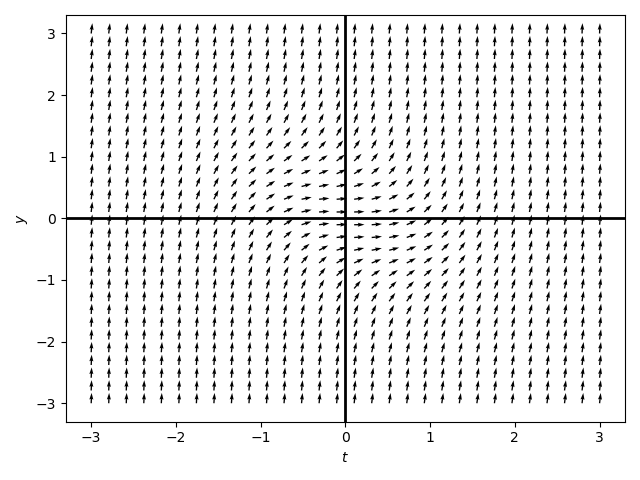
\includegraphics[width=6cm]{img/slope_field1.png}
		\caption{\label{fig:slope_field1} The Slope Field of $f(t, y)$ of Problem 1}
	\end{figure}
	
	In \autoref{fig:slope_field1} it seems that the solution curve of problem 1 is monotonic increasing. In fact, the derivative $y' = y^2 + ty + t^2 = (y + {1 \over 2}t)^2 + {3 \over 4}t^2 \geq 0$, thus it's globally increasing.
	
    Also, \autoref{fig:slope_field1} turns out that the maximal solution might be restricted between two vertical asymptotes. Therefore determining the domain is to determine these two essential asymptotes, and at this moment a using numerical method to make some attempts can be helpful.
    
    We make use of three numerical methods, i.e. the improved Euler method, the the fourth-order Runge-Kutta Method and the Adams-Moulton Method to determine the value of $t$ when $y$ is infinity.
    
    \begin{table}[H]
    \centering
    \resizebox{280pt}{!}{%
    \begin{tabular}{@{}lllllll@{}}
    \toprule
    \multicolumn{1}{l}{}           & \multicolumn{2}{c}{\textbf{Euler\_improved}}                       & \multicolumn{2}{c}{\textbf{RK\_4th}}                               & \multicolumn{2}{c}{\textbf{Adams-Moulton}}      \\ \midrule
    \multicolumn{1}{l}{\textbf{$h$}} & \multicolumn{1}{l}{\textbf{$a_1$}} & \multicolumn{1}{l}{\textbf{$b_1$}} & \multicolumn{1}{l}{\textbf{$a_1$}} & \multicolumn{1}{l}{\textbf{$b_1$}} & \multicolumn{1}{l}{\textbf{$a_1$}} & \multicolumn{1}{l}{\textbf{$b_1$}} \\ \hline
    0.01                           & -2.17                           & 0.91                            & -2.14                           & 0.88                            & -2.12                  & 0.85                   \\
    0.005                          & -2.15                           & 0.885                           & -2.13                           & 0.87                            & -2.1201                & 0.855                  \\
    0.001                          & -2.126                          & 0.864                           & -2.123                          & 0.861                           & -2.1202                & 0.858                  \\
    0.0005                         & -2.1235                         & 0.8615                          & -2.122                          & 0.86                            & -2.1205                & 0.8585                 \\
    0.0002                         & -2.1218                         & 0.86                            & -2.121                          & 0.8594                          & -2.1206                & 0.8587                 \\
    0.0001                         & -2.1212                         & 0.8594                          & -2.1209                         & 0.8591                          & -2.1207                & 0.8588                 \\ 
    \bottomrule
    \end{tabular}%
    }
    \caption{Determine t When y is Infinity}
    \label{tab:ivp1_inf_1}
    \end{table}
    
	It seems that the left bound of the solution is around $a_1 = -2.12$ and the right around $b_1 = 0.85$. To be more accurate, some analytical approaches should be adopted. 
	
	We will use two functions $f_1$ and $f_2$ to squeeze $f$ and reduce the range. The sign relationship between t and y should be determined first. We use the numerical results of the Adams-Moulton method at $t = -2.120$ and $t = 0.858$ in \autoref{tab:adams-monlton-domain-1} to illustrate some details.
	
    \begin{table}[H]
    \centering
    \resizebox{180pt}{!}{%
    \begin{tabular}{@{}lll@{}}
    \toprule
    \multicolumn{1}{l}{}           & \textbf{$t = -2.120$} & \textbf{$t = 0.858$} \\ \midrule
    \multicolumn{1}{l}{\textbf{$h$}} & \textbf{$y$}          & \textbf{$y$}         \\ \hline
    0.01                           & -\infty               & \infty           \\
    0.005                          & -\infty               & \infty           \\
    0.001                          & -\infty               & \infty           \\
    0.0005                         & -1657.12353516        & 1177.64002010    \\
    0.0002                         & -1523.43140641        & 1142.81318658     \\
    0.0001                         & -1518.10313846         & 1141.29183391   \\ \bottomrule
    \end{tabular}%
    }
    \caption{y of The Results of The Adams-Moulton Method When t = -2.120 And t = 0.858}
    \label{tab:adams-monlton-domain-1}
    \end{table}
    
    It's obvious that $t$ and $y$ have the same sign, plus the monotonicity and $|y| > |t|$ near the boundary, we can have such relationship: $y^2 < y^2 + ty + t^2 < 3y^2$. Therefore we obtain two solvable ODEs $y' = f_1(t, y) = y^2$ and $y' = f_2(t, y) = 3y^2$ to locate the boundary accurately. By solving these two ODEs we obtain:
    
    \begin{align}
        \Phi_1(t) &= -\frac{1}{t + C_1} \\
        \Phi_2(t) &= -\frac{1}{3t + C_2}
    \end{align}
    
    For the left boundary, we substitude the initial problem with $y(-2.120) = -1518.10313846$ from the results of \autoref{tab:adams-monlton-domain-1} and obtain $C_1 = 2.12065871$ and $C_2 = 6.36065871$, which turns out that the left bound should be restricted between $-2.12065871$ and $-2.12021957$, i.e., $-2.12065871 < a_1 < -2.12021957$.
    
    For the right boundary, similarly, we take the initial problem as $y(0.858) = 1141.29183391$ and obtain $C_1 = -0.85887620$ and $C_2 = -2.57487620$, which turns out that the right boundary should locate between $0.85829206$ and $0.85887620$, i.e., $0.85829206 < b_1 < 0.85887620$. 
	
	In conclusion, the domain of the solution of problem 1 is:
	
	$$
	\left\{
    	\begin{aligned}
    	    t &\in (a_1, b_1) \nonumber \\
    	    a_1 &\in (-2.12065871, -2.12021957) \nonumber \\
    	    b_1 &\in (0.85829206, 0.85887620) \nonumber
    	\end{aligned}
	\right.
	$$
	
		%______________________________________________
		
	\subsubsection{Problem 2: ($a_1$, $b_1$)}
	
    We start with the determination of the domain of solution. Same as problem 1, a slope field can be constructed to help understanding the tendency. According to the slope field \autoref{fig:slope_field2} shown below, the slopes seem not approach to infinite on the left side. Also, it seems that all the points below $y= -t$ have negative slope and all the points upon have positive slope. The numerical results of the improved Euler method in \autoref{tab:IVP2_y} also shows the tendency that it approaches to $y = -t$ when $t$ is approaching to negative infinity. 
	
	\begin{figure}[H]
		\centering
		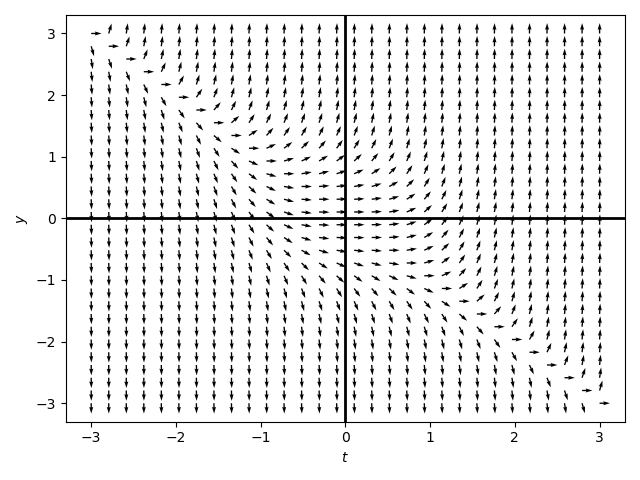
\includegraphics[width=6cm]{img/slope_field2.png}
		\caption{\label{fig:slope_field2} The Slope Field of $f(t, y)$ of Problem 2}
	\end{figure}
	
    \begin{table}[H]
    \centering
    \resizebox{350pt}{!}{%
    \begin{tabular}{@{}llllllllll@{}}
    \toprule
    \multicolumn{1}{c}{\textbf{t}} & \multicolumn{1}{c}{-50}     & \multicolumn{1}{c}{-45}        & \multicolumn{1}{c}{-40}        & \multicolumn{1}{c}{-35}        & \multicolumn{1}{c}{-30}         & \multicolumn{1}{c}{-25}         \\
    \midrule
    \multicolumn{1}{c}{\textbf{y}} & \multicolumn{1}{c}{49.9998} & \multicolumn{1}{c}{44.9997531} & \multicolumn{1}{c}{39.9996875} & \multicolumn{1}{c}{34.9995918} & \multicolumn{1}{c}{29.99944441} & \multicolumn{1}{c}{24.99919992} \\
     \bottomrule
    \end{tabular}%
    }
    \caption{Using Four Euler Method to Compute y Value}
    \label{tab:IVP2_y}
    \end{table}
    
    This qualitative tendency is proved as follows. Although \autoref{eq:ode2} is not an autonomous system, a "phase space" with $t$ as a parameter can still be constructed, as shown in the left-hand side in \autoref{fig:ivp2_phase}. The graph illustrates that the graph of $y' = f(y)$ has only one zero-crossing at $(-t, 0)$, and points near the line $y \equiv -t$ tend to go away from it (the blue arrows show the tendency), meaning this line is asymptotically unstable. In other words, if we go from $t = 0$ to $t = -\infty$, the sign of the derivative $y' = \frac{dy}{dt}$ should change, i.e. the graph becomes the right-hand side of \autoref{fig:ivp2_phase}, and the line $y \equiv -t$ now becomes an "asymptote". \\
    
    In addition, the solution $\Phi(t)$ with $t \rightarrow -\infty$ will approach to this "asymptote" from below, i.e., $\Phi(t) < -t$ with $t < \alpha$, where $\alpha$ is the point where the solution curve coincide with the line $y \equiv -t$. It is because $f_2(t, y)$ can be factorized as $y' = (y + t)(y^2 + t^2)$, making it obvious that the derivative of $\Phi(t)$ is negative if $\Phi(t) < -t$, positive if $\Phi(t) > -t$ and zero if $\Phi(t) = -t$. Therefore, the solution curve with $t < \alpha$ is restricted below the line $y \equiv -t$ because $\Phi(t)' < 0$. $t = \alpha$ is a turning point with $\Phi(\alpha)' = 0$ where the curve rises above $y \equiv -t$ since it should go through the initial condition $y(0) = 1$.
    
    \begin{figure}[H]
       \subfigure 
    {
    	\begin{minipage}{8cm}
    	 \centering      
    		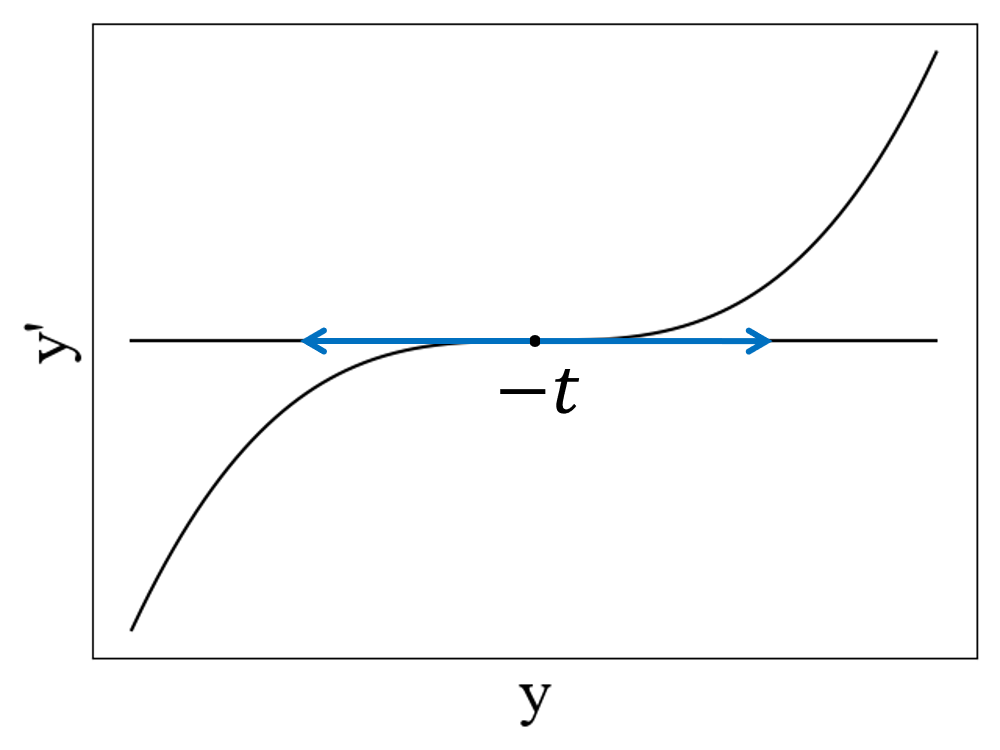
\includegraphics[width=6cm]{img/ivp2_phase_graph_1.png}
    		% \caption{\label{fig:ivp2_phase1}}
    	\end{minipage}
    }
      \subfigure 
    {
    	\begin{minipage}{8cm}
    	\centering      
    		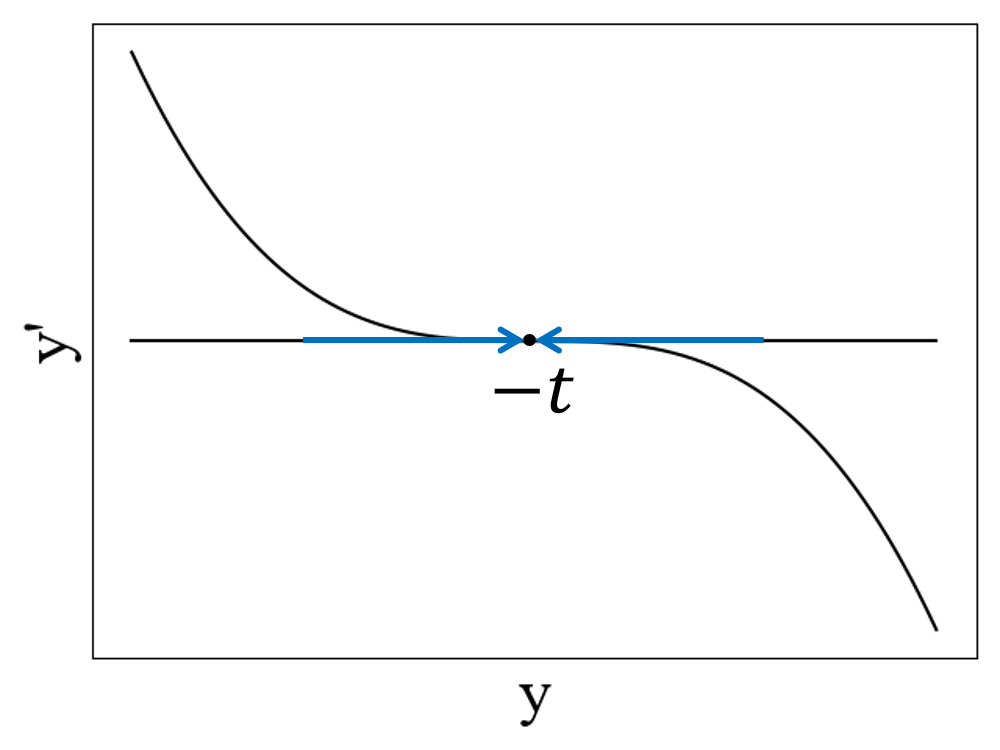
\includegraphics[width=6cm]{img/ivp2_phase_graph_2.png}
    		% \caption{\label{fig:ivp2_phase2} }
    	\end{minipage}
    }
    \caption{\label{fig:ivp2_phase} The Phase Space of \autoref{eq:ode2}} 
    \end{figure}
    
    Thus, the ODE does not have vertical asymptote on the left side. \\

    For the right vertical asymptote, we use four Euler methods to estimate. The value t is considered as stable location when the change of t value is less than 0.001 by one order step h reduction. The $t$ value where $y$ values first return inf from computation is considered as the approximate location of the vertical asymptote under that condition. Same as problem 1, a table can be constructed as \autoref{tab:IVP2_yinf}.
    
    \begin{table}[H]
    \centering
    \resizebox{400}{!}{%
    \begin{tabular}{@{}llllllllll@{}}
    \toprule
    \textbf{}           & \textbf{Euler\_explicit} & \textbf{Euler\_implicit} & \textbf{Euler\_improved} & \textbf{Euler\_trapezium} \\ 
    \hline
    \textbf{h = 0.01}   & 0.5                      & 0.4                      & 0.48                     & 0.43           \\
    \textbf{h = 0.005}  & 0.495                    & 0.42                     & 0.46                     & 0.435          \\
    \textbf{h = 0.001}  & 0.452                    & 0.436                    & 0.444                    & 0.44           \\ 
    \textbf{h = 0.0005} & 0.446                    & 0.438                    & 0.442                    & 0.4405          \\
    \textbf{h = 0.0002} & 0.4426                   & 0.4392                   & 0.4408                   & 0.4402         \\
    \textbf{h = 0.0001} & 0.4413                   & 0.4396                   & 0.4403                   & 0.4401   \\  
    \bottomrule                                       
    \end{tabular}%
    }
    \caption{Using Four Euler Methods to Compute The Nearest Value t Where y is Infinity }
    \label{tab:IVP2_yinf}
    \end{table}
 
	According to this numerical result, the difference of t is less than 0.001 when h = 0.0002 in both improved Euler method and trapezium Euler method’s calculation. Thus, t = 0.440 can be considered as the right vertical asymptote location of the ODE if only use the numerical methods. 
	
    \begin{table}[H]
    \centering
    \resizebox{300pt}{!}{%
    \begin{tabular}{@{}lllllll@{}}
    \toprule
    \textbf{h}          & 0.01 & 0.005 & 0.001       & 0.0005      & 0.0002      & 0.0001     \\ 
    \hline
    \textbf{y} & \infty  & \infty   & 25.62721138 & 23.60040387 & 23.43528374 & 23.4279037 \\ 
    \bottomrule
    \end{tabular}%
    }
    \caption{y of The Results of The Adams-Moulton Method When t = 0.439}
    \label{tab:adams-monlton-domain-2}
    \end{table}
	
	However, analytical approaches similar to problem 1 can still be adopted to acquire more accuracy. To illustrate the details and relationship between $t$ and $y$ we use the Adams-Moulton method at $t = 0.439$ again. Obviously, near the right border $t$ and $y$ are both positive and $y > t$, therefore, we can obtain such an relationship: $y^3 < y^3 + ty^2 +t^2y +t^3 < 4y^3$, which consists of two solvable ODEs $y' = f_1(t, y) = y^3$ and $y' = f_2(t, y) = 4y^3$. By solving them we obtain:
	
	\begin{align}
	    \Phi_1(t) &= \frac{1}{\sqrt{2}\sqrt{C_1 - t}} \\
	    \Phi_2(t) &= \frac{1}{\sqrt{2}\sqrt{C_2 - 4t}}
	\end{align}
	
	Now we can choose one pair of $(t, y)$ from \autoref{tab:adams-monlton-domain-2} as a new initial value. we take $y(0.439) = 23.4279037$ and obtain $C_1 = 0.4399109$ and $C_2 = 1.7569109$, which leads to the results that the right boundary of problem 2 should locate between $0.4392277$ and $0.4399109$, i.e., $0.4392277 < b_2 < 0.4399109$.
	
	In conclusion, the domain of the solution of problem 2 is:
	
	$$
	\left\{
    	\begin{aligned}
    	    t &\in (-\infty, b_2) \nonumber \\
    	    b_2 &\in (0.4392277, 0.4399109) \nonumber
    	\end{aligned}
	\right.
	$$

	%_____________________________________________

    
    \subsection{Accuracy}
    To judge whether a method is good or not, the accuracy is one of the most important factor. We define the error of a result of a certain method with certain stepsize at a certain point $t$ as $|\hat{y} - y|$, where $\hat{y}$ is the numerical result and $y$ is the accurate solution. 
    
    Here we mainly study about two questions: How does the error change with different h for one certain method? Which method is more accurate when stepsize h is fixed? We will control variables to do the research below. For a certain method, the relationship between the stepsize $h$ and the error should first be estimated.
    
    \begin{figure}[H]
    \centering
    \subfigure{
    \begin{minipage}[t]{0.2\linewidth}
    \centering
    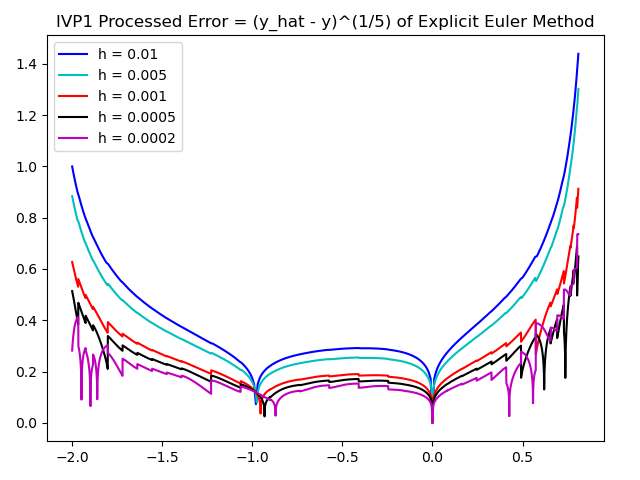
\includegraphics[width=1.5in]{img/ivp1_error_h_euler_explicit.png}
    %\caption{fig1}
    \end{minipage}%
    }
    \subfigure{
    \begin{minipage}[t]{0.2\linewidth}
    \centering
    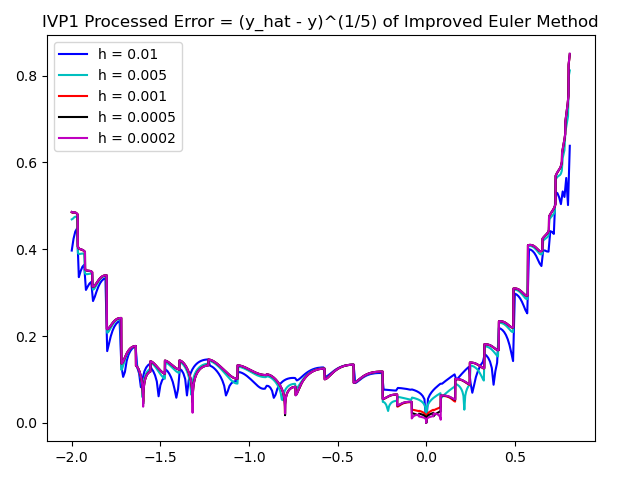
\includegraphics[width=1.5in]{img/ivp1_error_h_euler_improved.png}
    %\caption{fig2}
    \end{minipage}%
    }%
    \subfigure{
    \begin{minipage}[t]{0.2\linewidth}
    \centering
    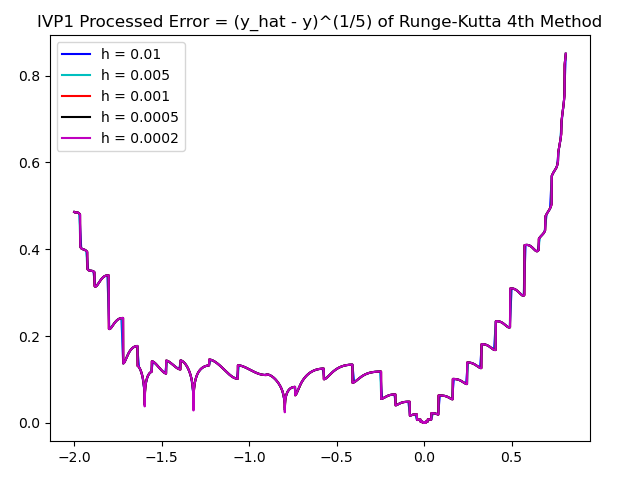
\includegraphics[width=1.5in]{img/ivp1_error_h_rk4.png}
    %\caption{fig2}
    \end{minipage}
    }%
    \subfigure{
    \begin{minipage}[t]{0.2\linewidth}
    \centering
    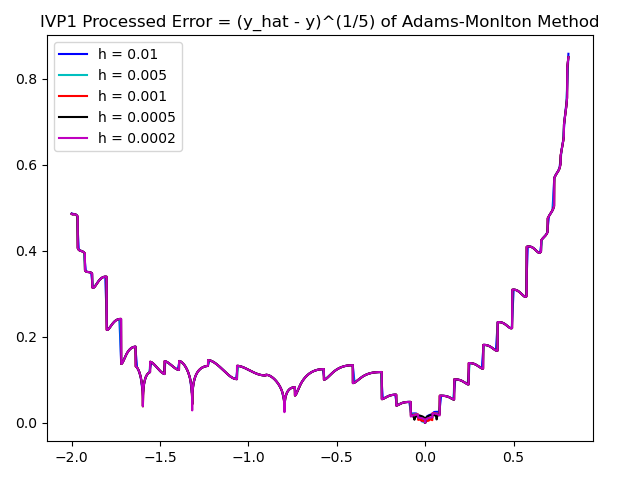
\includegraphics[width=1.5in]{img/ivp1_error_h_adams_monlton.png}
    %\caption{fig2}
    \end{minipage}
    }%
    \centering
    \caption{Error with Different h of Four Methods in IVP1}
    \end{figure}
       %%%%%%%____________________________________________________________
       
    \begin{figure}[H]
    \centering
    \subfigure{
    \begin{minipage}[t]{0.2\linewidth}
    \centering
    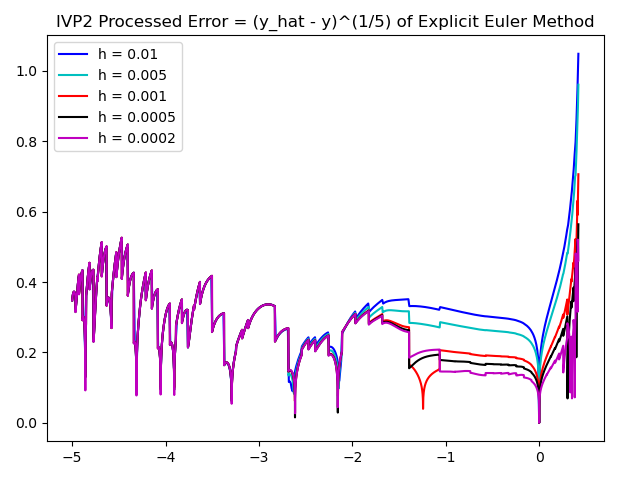
\includegraphics[width=1.5in]{img/ivp2_error_h_euler_explicit.png}
    %\caption{fig1}
    \end{minipage}%
    }
    \subfigure{
    \begin{minipage}[t]{0.2\linewidth}
    \centering
    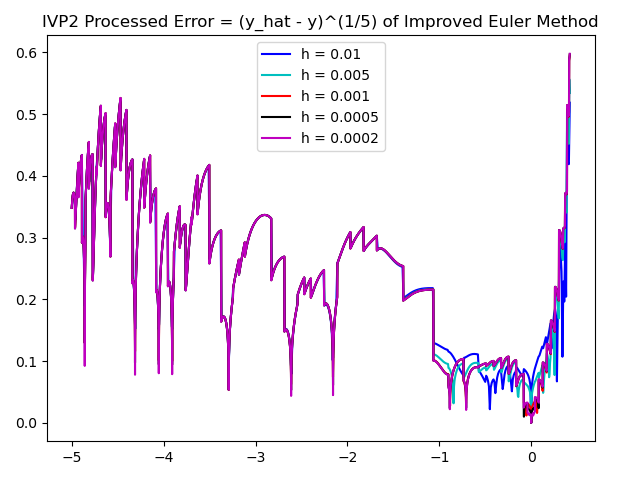
\includegraphics[width=1.5in]{img/ivp2_error_h_euler_improved.png}
    %\caption{fig2}
    \end{minipage}%
    }%
    \subfigure{
    \begin{minipage}[t]{0.2\linewidth}
    \centering
    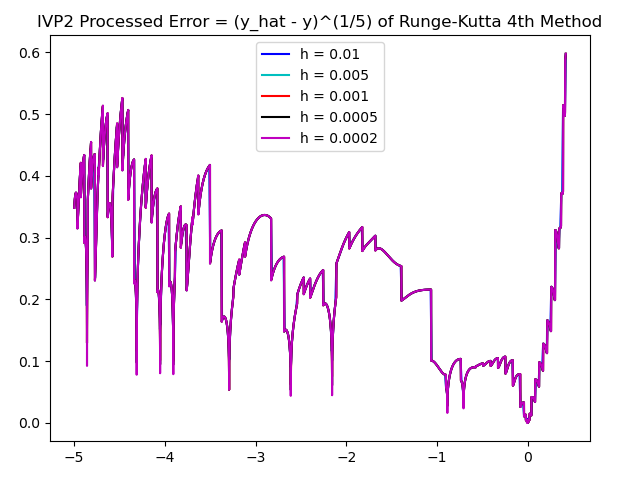
\includegraphics[width=1.5in]{img/ivp2_error_h_rk4.png}
    %\caption{fig2}
    \end{minipage}
    }%
    \subfigure{
    \begin{minipage}[t]{0.2\linewidth}
    \centering
    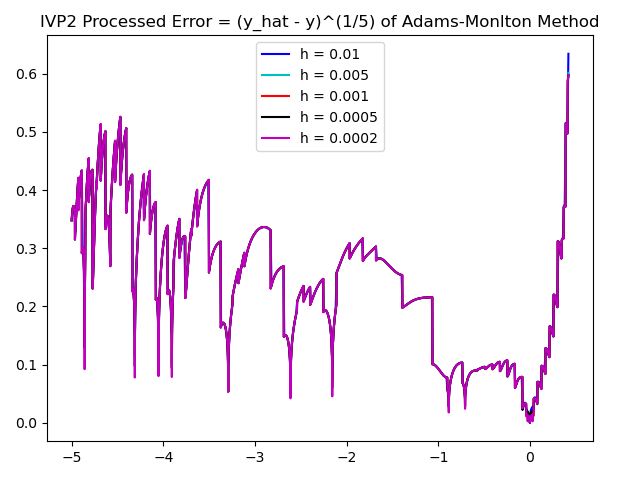
\includegraphics[width=1.5in]{img/ivp2_error_h_adams_monlton.png}
    %\caption{fig2}
    \end{minipage}
    }%
    \centering
    \caption{Error with Different h of Four Methods in IVP2}
    \end{figure}
   
    From the above graphs we can see, for all these methods, the numerical solutions will be more accurate with the step size h decreasing in a certain range. 
    
    \subsubsection{The Errors with Same h in Different Methods}
    
    The second part is the accuracy comparison among different methods. For this problem the error comparison graphs of IVP1 and IVP2 are to be made. 
    From the conclusion above, it is already known that error and $h$ are positive correlated for all these methods. So here we just use $h = 0.01$ to continue the research below. 
    Because the largest error and smallest error differs largely, we take the errors to the root three times or four times to better compare in one graph, which brings those large numbers and small numbers closer to 1 and makes the curves more distinguishable.
    
   From the first graph of IVP1 below, we can get that the error of the explicit Euler method is the largest. With a $h=0.01$, the errors of the other four methods are quite similar. 
   For IVP2, the error of the explicit Euler method is the largest as well. The improved Euler method has the second largest error. Other methods have quite similar errors.
   All in all, the Adams-Moulton method is the most accurate and the Euler method has the largest error. The errors of the improved Euler method, the trapezium Euler method and the Runge-Kutta method are quite similar. 
   
     %two graphs in same line  
    \begin{figure}[H]
    \subfigure 
    {
    	\begin{minipage}{8cm}
    	 \centering      
    		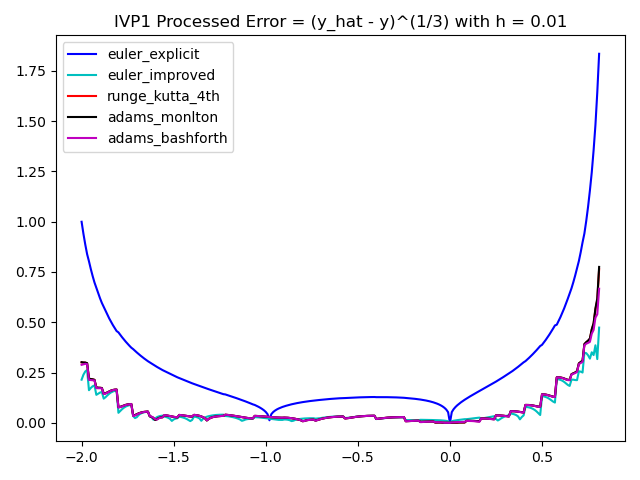
\includegraphics[width=7.5cm]{img/ivp1_error.png}
    		\caption{\label{fig:ivp1_error} }
    	\end{minipage}
    }
    \subfigure 
    {
    	\begin{minipage}{8cm}
    	\centering      
    		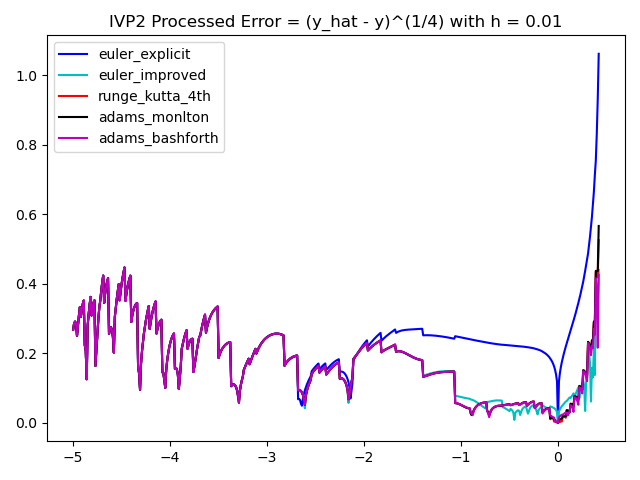
\includegraphics[width=7.5cm]{img/ivp2_error.png}
    		\caption{\label{fig:ivp2_error}}
    	\end{minipage}
    }
    \caption{Error Comparison Graphs of IVP1, IVP2} 
    \end{figure}
   
   In theoretical, the global truncation error of each method is different because of the formula inside. For the Euler method, the global truncation error is proportional to the 1st power of h, so the error might be the largest among these methods. For the improved Euler method, the global truncation error is proportional to the 2nd power of h. The fourth-order four-stage Runge-Kutta method has a global truncation error of $h^4$. The Adams-Moulton method has a global truncation error of $h^5$.
   
   From this comparison graph another conclusion come into being: it is not the case that the more accurate a method is, the better it is. Since the fourth-order Runge-Kutta method has a global truncation error of $h^4$ and the improved Euler method has a global truncation error of $h^3$, while they have quite close solutions. So accuracy is not the only factor we need to consider, to judge whether a method is suitable or not for one ODE, we need to consider if it is worthwhile spending much more time on calculation to increase only very small amount of accuracy. 
   
   In this case, computation complexity should also be considered.
   
     %_____________________________________________
     
    \subsection{Complexity}
    In general, "Computation Complexity" can be composed of "Time Complexity" and "Space Complexity ". Since the two can convert to each other and in numerical methods the intermediate processes of each method mainly have effect on the total time. So time complexity will be the main part discussed here.
    
    % \usepackage{booktabs}
    % \usepackage{graphicx}
    \begin{table}[H]
    \centering
    \resizebox{\textwidth}{!}{%
    \begin{tabular}{@{}lllllllll@{}}
    \toprule
    \textbf{h} & \textbf{Euler\_explicit} & \textbf{Euler\_implicit} & \textbf{Euler\_trape} & \textbf{Euler\_imprd} & \textbf{RK\_3rd} & \textbf{RK\_4th} & \textbf{Adams\_moulton} & \textbf{Adams\_bashforth} \\ \midrule
    0.01       & 0.199389648              & 3.893579102            & 3.191479492           & 0.398876953           & 0.498486328      & 0.797802734      & 22.0447998            & 1.19675293               \\
    0.005      & 0.39909668               & 6.683203125            & 6.183374023           & 0.797827148           & 1.097021484      & 1.495996094      & 43.6833252            & 2.393554688              \\
    0.001      & 1.996264648              & 29.11706543            & 30.41862793           & 4.089111328           & 5.485375977      & 7.830151367      & 197.6515381           & 14.06235352              \\
    0.0005     & 3.889575195              & 54.87087402            & 54.06862793           & 8.577001953           & 10.9706543       & 15.75786133      & 406.0815674           & 29.12207031              \\
    0.0002     & 10.27258301              & 143.0174561            & 132.257959            & 19.64763184           & 27.33054199      & 40.19226074      & 955.9131592           & 63.23076172              \\
    0.0001     & 24.43808594              & 290.3356445            & 232.636792            & 38.99562988           & 56.57814941      & 85.29304199      & 1956.909473           & 143.8662109              \\ \bottomrule
    \end{tabular}%
    }
    \caption{Time Consuming  with Different h in IVP1}
    \label{tab:IVP1}
    \end{table}
    
    % \usepackage{booktabs}
    % \usepackage{graphicx}
    \begin{table}[H]
    \centering
    \resizebox{\textwidth}{!}{%
    \begin{tabular}{@{}lllllllll@{}}
    \toprule
    \textbf{h} & \textbf{Euler\_explicit} & \textbf{Euler\_implicit} & \textbf{Euler\_trape} & \textbf{Euler\_improved} & \textbf{RK\_3rd} & \textbf{RK\_4th} & \textbf{Adams\_moulton} & \textbf{Adams\_bashforth} \\ \midrule
    0.01       & 1.19260254            & 48.57026367              & 43.97243652           & 2.78720703               & 3.49047852       & 5.28737793       & 315.6517334           & 6.38789062                \\
    0.005      & 2.59301758            & 59.17590332              & 48.36687012           & 5.88430176               & 7.67946777       & 10.57209473      & 443.2843994           & 13.06520996               \\
    0.001      & 12.9652832            & 30.43623047              & 33.61003418           & 30.71765137              & 41.64165039      & 54.85251465      & 493.8230713           & 66.11806641               \\
    0.0005     & 28.42741699           & 54.05429687              & 67.07429199           & 61.84191895              & 77.99611816      & 109.7824219      & 806.3147949           & 132.3153076               \\
    0.0002     & 75.06044922           & 140.6254883              & 178.127832            & 160.380542               & 198.1198486      & 261.8647461      & 1660.448975           & 337.3976074               \\
    0.0001     & 162.1139404           & 289.7324219              & 379.6040283           & 339.4297119              & 399.6322754      & 538.4823975      & 3068.49563            & 685.1721191               \\ \bottomrule
    \end{tabular}%
    }
    \caption{Time Consuming  with Different h in IVP2}
    \label{tab:IVP2}
    \end{table}
    
    For one certain method, time consuming increases with the stepsize h getting smaller. This makes sense since smaller h will lead to more steps of calculation.
    
    When comparing time consuming among different methods, some rules come out.
    Firstly, the Euler method costs least time to finish the calculation. It has the advantage that the formula is simple and easy to run in computer. 
    For both two IVP problems, the computation complexity of the improved Euler method’s algorithm increases compared to the Euler method, since $f(t,y)$ should be evaluated twice in the formula to go from $t_n$ to $t_n+1$ in the formula. But the improved Euler method still cost little time in total.
    The fourth-order four-stage Runge-Kutta method, weighing four steps with ${1\over6}(k_{n1}+2k_{n2}+2k_{n3}+k_{n4})$. An increasing in accuracy will lead to a more complex algorithm.
    The Adams-Moulton method and the Adams-Bashforth method are multi-step methods, it would take more time to evaluate.
    
    Another important discovery is that the implicit Euler method, the trapezium Euler method and the Adams-Moulton method have obviously larger errors than the others. This is because these methods are implicit and the operation process is iterative. Especially for the Adams-Moulton method, the iteration is much more complicated than the others. So the Adams-Moulton method is the most time consuming.
    
    In theoretical, using a "Big-O" method to evaluate these methods, the conclusion is that all methods are in the order of $O(mn)\in{O(n)}$,$m\in{O(1)}$. When n goes infinite, all of these methods may cost the same time. 
    
    In a certain range, there exists a negative correlation between computation complexity and accuracy. However, this is not always true.
    
    In addition, the time consuming might also influenced by the detailed ODE functions. For example, the Adams-Bashforth method costs less time than the implicit Euler method for IVP1 problem but costs more time than the implicit Euler method for IVP2.
    
    %_____________________________________________
    
    \section{Conclusion}
    
	Usually a high accuracy method would cost more time and space to get the solution, however, within the tolerable margin of error, a simpler method would be more suggested.
	
	In a conclusion, every method has its own merit and demerit.	
	In reality Which one to choose should depend more on the detailed ODE function and the balance between accuracy and computation complexity requirements.
	
	%_____________________________________________
	
    \clearpage

    \begin{appendices}
    
    \section{Power Series Solution}\label{apdx:power_series}
    
    \subsection{Problem 1}
    
    Substituting the power series "Ansatz" $y(t) = \sum_{n=0}^{\infty} a_n t^n$ to \autoref{eq:ode1}, we will have:
    
    \begin{equation}
        \sum_{n=1}^{\infty} n a_n t^{n-1} = t^2 + \sum_{n = 0}^{\infty}(\sum_{k=0}^{n}a_k a_{n-k})t^n + \sum_{n=0}^{\infty}a_n t^{n+1}
    \end{equation}
    
    that is, 
    
    \begin{equation}
        a_1 - t^2 = \sum_{n=0}^{\infty}(\sum_{k=0}^{n}a_k a_{n-k})t^n + \sum_{n=1}^{\infty}(a_{n-1}-(n+1)a_{n+1})t^n
    \end{equation}
    
    which after reorganizing is, 
    
    \begin{equation}
        \sum_{n=1}^{\infty}((n+1)a_{n+1} - a_{n-1})t^n = t^2 - a_1 + \sum_{n=1}^{\infty}(\sum_{k=0}^{n}a_k a_{n-k})t^n + a_0 a_n
    \end{equation}
    
    Which can be reorganized as
    
    \begin{equation}
        \begin{cases}
            (n+1)a_{n+1}-a_{n-1} = 
                \begin{cases}
                    \sum_{k=0}^{n-k}a_k a_{n-k}, & \text{$n \neq 2$} \\
			    	2a_0a_n + a_1^2 + 1, & \text{$n = 2$} \\
                \end{cases} \\
            a_0 a_n - a_1 = 0 \\
            a_0 = a_1 = 1
        \end{cases}
    \end{equation}
    
    Therefore, we obtain a recursion relationship as:
    
    \begin{equation}
        \begin{cases}
            a_0 = 1 \\
            a_1 = 1 \\
            2a_2 - 3a_3 + 3 = 0 \\
            a_n = 1 \\
            (n+1)a_{n+1}-a_{n-1} = \sum_{k=0}^{n-k}a_k a_{n-k}, & \text{$n > 2$} \\
        \end{cases}
    \end{equation}
    
    \subsection{Problem 2}
    
    Similar to problem 1, we substitude the power series "Ansatz" $y(t) = \sum_{n=0}^{\infty} a_n t^n$ to \autoref{eq:ode1}, we will have:
    
    \begin{equation}
        \sum_{n=1}^{\infty} n a_n t^{n-1} = \sum_{n=0}^{\infty}(\sum_{i=0}^{n}(\sum_{j=0}^{i}a_j a_{i-j} a_{n-i})) t^n + \sum_{n=0}^{\infty}(\sum_{k=0}^{n}a_k a_{n-k})t^{n+1} + \sum_{n=0}^{\infty} a_{n} t^{n+2} + t^3
    \end{equation}
    
    Which is, after reorganizing, 
    
    \begin{equation}
        a_1 + 2a_2t + \sum_{n=2}^{\infty}(n+1)a_{n+1}t^n = a_0^3 + (3a_0^2 a_1 + 2a_0 a_1)t + t^3 + \sum_{n=2}^{\infty}(\sum_{i=0}^n(\sum_{j=0}^i a_j a_{i-j} a_{n-i}) + \sum_{k=0}^n a_k a_{n-k} + a_{n+2}) t^n
    \end{equation}
    
    That is, 
    
    \begin{equation}
        \begin{cases}
            (n+1)a_{n+1} = 
                \begin{cases}
                    \sum_{i=0}^{n}(\sum_{j=0}^{i}a_j a_{i-j} a_{n-i}) + \sum_{k=0}^{n} a_K a_{n-k} + a_{n+2}, & \text{$n \neq 3$} \\
			    	\sum_{i=0}^{n}(\sum_{j=0}^{i}a_j a_{i-j} a_{n-i}) + \sum_{k=0}^{n} a_K a_{n-k} + a_{n+2} + 1, & \text{$n = 3$} \\
                \end{cases} \\
            a_1 - a_0^3 = 0 \\
            3a_0^2 a_1 + 2a_0 a_1 - 2a_2 = 0 \\
            a_0 = a_1 = 1
        \end{cases}
    \end{equation}
    
    Therefore, we obtain a recursion relationship as:
    
    \begin{equation}
        \begin{cases}
            a_0 = 1 \\
            a_1 = 1 \\
            a_2 = {5 \over 2} \\
            a_5 - 4a_4 + 5a_3 + 22 = 0 \\
            (n+1)a_{n+1} = \sum_{i=0}^{n}(\sum_{j=0}^{i}a_j a_{i-j} a_{n-i}) + \sum_{k=0}^{n} a_k a_{n-k} + a_{n+2}, & \text{$n > 3$} \\
        \end{cases}
    \end{equation}
    
    \clearpage
    
    \section{Code} \label{apdx:code}
    
    All the code and numerical solutions are open source on the GitHub repository \href{https://github.com/RickyL-2000/math286_lab}{RickyL-2000/math286\_lab}.
    
    \subsection{Generation of Accurate Solution (MatLab)}
    
    \begin{lstlisting} [language=MatLab]
    %%% problem 1 %%%
    tspan1 = [0:-0.0001:-2.12];
    y0 = 1;
    [t1,y1] = ode113(@(t,y) y^2+y*t+t^2, tspan1, y0);
    k = flipud([t1,y1]);
    tspan2 = [0:0.001: 0.858];
    [t2,y2] = ode113(@(t,y) y^2+y*t+t^2, tspan2, y0);
    j = [t2,y2];
    j(1, :) = [];
    n=[k; j];
    result_table = table(n(:,1), n(:,2));
    writetable(result_table, 'ivp1_ground_truth.csv')
    
    %%%% problem 2 %%%
    tspan3 = [0:-0.001:-25];
    y0 = 1;
    [t3,y3] = ode113(@(t,y) y^3+y*t^2+t*y^2+t^3, tspan3, y0);
    kk = flipud([t3,y3]);
    tspan4 = [0:0.0001: 0.439];
    [t4,y4] = ode113(@(t,y) y^3+y*t^2+t*y^2+t^3, tspan4, y0);
    jj = [t4,y4];
    jj(1,:) = [];
    nn = [kk; jj];
    result_table = table(nn(:,1), nn(:,2));
    writetable(result_table, 'ivp2_ground_truth.csv')
    
    \end{lstlisting}
    
    \clearpage
    
    \subsection{The Euler Method (Python)}
    
    \begin{lstlisting} [language=Python]
    import pandas as pd
    import numpy as np
    
    def euler_explicit(f, a, b, t0, y0, h) -> Tuple[np.ndarray, np.ndarray]:
        """
        Explicit Euler Method
    
        :param f: the f function
        :param a: left bound
        :param b: right bound
        :param t0: initial t
        :param y0: initial y
        :param h: step length
        :return: list of numerical results of t and y
        """
        assert a <= t0 <= b
        t_list, y_list = [], []
        ti, yi = t0, y0
        t_temp, y_temp = [], []
        for _ in range(round((t0 - a)/h)):
            y_ = yi - h * f(ti, yi)
            t_temp.append(ti-h), y_temp.append(y_)
            ti, yi = ti-h, y_
    
        if t_temp and y_temp:
            t_temp.reverse(), y_temp.reverse()
            t_list.extend(t_temp), y_list.extend(y_temp)
    
        t_list.append(t0), y_list.append(y0)
    
        ti, yi = t0, y0
        # while ti+h <= b:
        for _ in range(round((b - t0)/h)):
            y_ = yi + h * f(ti, yi)
            t_list.append(ti+h), y_list.append(y_)
            ti, yi = ti+h, y_
    
        return np.array(t_list), np.array(y_list)
    
    def euler_implicit(f, a, b, t0, y0, h, threshold=1e-6, epochs=100) -> Tuple[np.ndarray, np.ndarray]:
        """
        Implicit (backward) Euler Method

        :param threshold: the threshold to control the iteration
        :param epochs: the maximum number of epochs used to control the iteration
        :return: list of numerical results of t and y
        """
        assert a <= t0 <= b
        t_list, y_list = [], []
        ti, yi = t0, y0
        t_temp, y_temp = [], []
        for _ in range(round((t0 - a)/h)):
            y_ = yi - h * f(ti, yi)
            epoch = 0
            while True:
                epoch += 1
                y__ = yi - h * f(ti-h, y_)
                if abs(y__ - y_) < threshold or epoch > epochs:
                    break
                y_ = y__
            t_temp.append(ti-h), y_temp.append(y_)
            ti, yi = ti-h, y_
    
        if t_temp and y_temp:
            t_temp.reverse(), y_temp.reverse()
            t_list.extend(t_temp), y_list.extend(y_temp)
    
        t_list.append(t0), y_list.append(y0)
    
        ti, yi = t0, y0
        for _ in range(round((b - t0) / h)):
            y_ = yi + h * f(ti, yi)
            epoch = 0
            while True:
                epoch += 1
                y__ = yi + h * f(ti + h, y_)
                if abs(y__ - y_) < threshold or epoch > epochs:
                    break
                y_ = y__
            t_list.append(ti + h), y_list.append(y_)
            ti, yi = ti + h, y_
    
        return np.array(t_list), np.array(y_list)
    
    def euler_trapezium(f, a, b, t0, y0, h, threshold=1e-6, epochs=50) -> Tuple[np.ndarray, np.ndarray]:
        """
        Implicit (backward) Euler Method
    
        :param threshold: the threshold to control the iteration
        :param epochs: the maximum number of epochs used to control the iteration
        :return: list of numerical results of t and y
        """
        assert a <= t0 <= b
        t_list, y_list = [], []
        ti, yi = t0, y0
        t_temp, y_temp = [], []
        for _ in range(round((t0 - a) / h)):
            y_ = yi - h * f(ti, yi)
            epoch = 0
            while True:
                epoch += 1
                y__ = yi - 0.5 * h * (f(ti, yi) + f(ti - h, y_))
                if abs(y__ - y_) < threshold or epoch > epochs:
                    break
                y_ = y__
            t_temp.append(ti - h), y_temp.append(y_)
            ti, yi = ti - h, y_
    
        if t_temp and y_temp:
            t_temp.reverse(), y_temp.reverse()
            t_list.extend(t_temp), y_list.extend(y_temp)
    
        t_list.append(t0), y_list.append(y0)
    
        ti, yi = t0, y0
        for _ in range(round((b - t0) / h)):
            y_ = yi + h * f(ti, yi)
            epoch = 0
            while True:
                epoch += 1
                y__ = yi + 0.5 * h * (f(ti, yi) + f(ti + h, y_))
                if abs(y__ - y_) < threshold or epoch > epochs:
                    break
                y_ = y__
            t_list.append(ti + h), y_list.append(y_)
            ti, yi = ti + h, y_
    
        return np.array(t_list), np.array(y_list)
    
    def euler_improved(f, a, b, t0, y0, h) -> Tuple[np.ndarray, np.ndarray]:
        """
        Improved Euler Method
        """
        assert a <= t0 <= b
        t_list, y_list = [], []
        ti, yi = t0, y0
        t_temp, y_temp = [], []
        for _ in range(round((t0 - a)/h)):
            y_ = yi - h * f(ti, yi)
            y_ = yi - 0.5 * h * (f(ti, yi) + f(ti-h, y_))
            t_temp.append(ti-h), y_temp.append(y_)
            ti, yi = ti-h, y_
        if t_temp and y_temp:
            t_temp.reverse(), y_temp.reverse()
            t_list.extend(t_temp), y_list.extend(y_temp)
    
        t_list.append(t0), y_list.append(y0)
    
        ti, yi = t0, y0
        for _ in range(round((b - t0)/h)):
            y_ = yi + h * f(ti, yi)
            y_ = yi + 0.5 * h * (f(ti, yi) + f(ti+h, y_))
            t_list.append(ti+h), y_list.append(y_)
            ti, yi = ti+h, y_
    
        return np.array(t_list), np.array(y_list)

    \end{lstlisting}
    
    \clearpage
    
    \subsection{The Runge-Kutta Method (Python)}
    
    \begin{lstlisting} [language=Python]
    import pandas as pd
    import numpy as np
    def runge_kutta_3rd(f, a, b, t0, y0, h, **params) -> Tuple[np.ndarray, np.ndarray]:
        """
        3-order-Runge Kutta method
        :param f: the f function
        :param a: left bound
        :param b: right bound
        :param t0: initial t
        :param y0: initial y
        :param h: step length
        :param params: params to be determined, should contain 'alpha' and 'beta' tuples.
                       default: kwargs['alpha'] = (1/6, 2/3, 1/6);
                                kwargs['beta'] = (1/2, 1/2, 1.0, -1.0, 2.0)
        :return: list of numerical results of t and y
        """
        assert a <= t0 <= b
    
        if 'alpha' in params:
            alpha = params['alpha']
        else:
            alpha = (1/6, 2/3, 1/6)
        if 'beta' in params:
            beta = params['beta']
        else:
            beta = (1/2, 1/2, 1.0, -1.0, 2.0)
    
        assert equal(sum(alpha), 1.0)
        assert equal(beta[0] * alpha[1] + beta[2] * alpha[2], 0.5)
        assert equal(beta[2], beta[3] + beta[4])
        assert equal(beta[0], beta[1])
        assert equal(beta[0] * beta[0] * alpha[1] + beta[2] * beta[2] * alpha[2], 1/3)
        assert equal(beta[0] * beta[4] * alpha[2], 1/6)
    
        t_list, y_list = [], []
        ti, yi = t0, y0
        t_temp, y_temp = [], []
        for _ in range(round((t0 - a)/h)):
            k1 = h * f(ti, yi)
            k2 = h * f(ti - beta[0]*h, yi - beta[1]*k1)
            k3 = h * f(ti - beta[2]*h, yi - beta[3]*k1 - beta[4]*k2)
            y_ = yi - alpha[0] * k1 - alpha[1] * k2 - alpha[2] * k3
            t_temp.append(ti-h)
            y_temp.append(y_)
            ti, yi = ti-h, y_
        if t_temp and y_temp:
            t_temp.reverse(), y_temp.reverse()
            t_list.extend(t_temp), y_list.extend(y_temp)
    
        t_list.append(t0), y_list.append(y0)
    
        ti, yi = t0, y0
        for _ in range(round((b - t0)/h)):
            k1 = h * f(ti, yi)
            k2 = h * f(ti + beta[0] * h, yi + beta[1] * k1)
            k3 = h * f(ti + beta[2] * h, yi + beta[3] * k1 + beta[4] * k2)
            y_ = yi + alpha[0] * k1 + alpha[1] * k2 + alpha[2] * k3
            t_list.append(ti+h)
            y_list.append(y_)
            ti, yi = ti + h, y_
    
        return np.array(t_list), np.array(y_list)
    
    def runge_kutta_4th(f, a, b, t0, y0, h, **params) -> Tuple[np.ndarray, np.ndarray]:
        """
        4-order-Runge Kutta method
    
        :param f: the f function
        :param a: left bound
        :param b: right bound
        :param t0: initial t
        :param y0: initial y
        :param h: step length
        :param params: params to be determined, should contain 'alpha' and 'beta' tuples.
                       default: kwargs['alpha'] = (1/6, 1/3, 1/3, 1/6);
                                kwargs['beta'] = (1/2, 1/2, 1/2, 0, 1/2, 1, 0, 0, 1)
        :return: list of numerical results of t and y
        """
        # NOTE: The check of the parameters are too sophisticated so just skip it
    
        if 'alpha' in params:
            alpha = params['alpha']
        else:
            alpha = (1/6, 1/3, 1/3, 1/6)
        if 'beta' in params:
            beta = params['beta']
        else:
            beta = (1/2, 1/2, 1/2, 0, 1/2, 1, 0, 0, 1)
    
        t_list, y_list = [], []
        ti, yi = t0, y0
        t_temp, y_temp = [], []
        for _ in range(round((t0 - a) / h)):
            k1 = h * f(ti, yi)
            k2 = h * f(ti - beta[0] * h, yi - beta[1] * k1)
            k3 = h * f(ti - beta[2] * h, yi - beta[3] * k1 - beta[4] * k2)
            k4 = h * f(ti - beta[5] * h, yi - beta[6] * k1 - beta[7] * k2 - beta[8] * k3)
            y_ = yi - alpha[0] * k1 - alpha[1] * k2 - alpha[2] * k3 - alpha[3] * k4
            t_temp.append(ti - h)
            y_temp.append(y_)
            ti, yi = ti - h, y_
        if t_temp and y_temp:
            t_temp.reverse(), y_temp.reverse()
            t_list.extend(t_temp), y_list.extend(y_temp)
    
        t_list.append(t0), y_list.append(y0)
    
        ti, yi = t0, y0
        for _ in range(round((b - t0) / h)):
            k1 = h * f(ti, yi)
            k2 = h * f(ti + beta[0] * h, yi + beta[1] * k1)
            k3 = h * f(ti + beta[2] * h, yi + beta[3] * k1 + beta[4] * k2)
            k4 = h * f(ti + beta[5] * h, yi + beta[6] * k1 + beta[7] * k2 + beta[8] * k3)
            y_ = yi + alpha[0] * k1 + alpha[1] * k2 + alpha[2] * k3 + alpha[3] * k4
            t_list.append(ti + h)
            y_list.append(y_)
            ti, yi = ti + h, y_
    
        return np.array(t_list), np.array(y_list)

    \end{lstlisting}
    
    \clearpage
    
    \subsection{The Adams Method (Python)}
    
    \begin{lstlisting} [language=Python]
    import numpy as np
    from lab.euler import euler_trapezium, euler_improved, euler_implicit, euler_explicit
    from lab.runge_kutta import runge_kutta_4th, runge_kutta_3rd

    def lin_multistep(f, a, b, t0, y0, h, **kwargs) -> Tuple[np.ndarray, np.ndarray]:
        """
        The general linear multi-step method
    
        :param f: the f function
        :param a: left bound
        :param b: right bound
        :param t0: initial t
        :param y0: initial y
        :param h: the step length (**can be negative to predict the left part**)
        :param kwargs: params to be determined.
                        default:
                        k: number of steps, k=3;
                        alpha: the first set of params, alpha=(1, 0, 0);
                        beta: the second set of params, beta=(0, 23/12, -4/3, 5/12);
                        pre_method: the method to predict the points within the k steps, pre_method=runge_kutta_4th;
                        threshold: the threshold to control the iteration of implicit part, threshold=1e-4;
                        epochs: the upper bound of the epochs to iter to 
                                control the iteration of implicit part, epochs=100;
        :return: list of numerical results of t and y
        """
    
        def __update(t_list: List, y_list: List, f_list: List, f, h: float, k: int, alpha: Tuple, beta: Tuple,
                     threshold=1e-6, epochs=100) -> float:
            """
            Choose to whether update the y_{i+1} explicitly or implicitly
    
            :param t_list: the current t_i sequence (the t_{i+1} is to be predicted) 
                                                    (can be reversed to predict the left part)
            :param y_list: the current y_i sequence (the y_{i+1} is to be predicted) 
                                                    (can be reversed to predict the left part)
            :param h: the step length (**can be negative to predict the left part**)
            :param threshold: the threshold to control the iteration of implicit part
            :param epochs: the upper bound of the epochs to iter to control the iteration of implicit part
            :return: the new numerical result of y_{i+1}
            """
            if beta[0] == 0:
                # explicit
                return sum([alpha[i] * y_list[-i - 1] for i in range(k)]) + \
                       h * sum([beta[i+1] * f_list[-i - 1] for i in range(k)])
            else:
                # implicit
                epoch = 0
                y_ = sum([alpha[i] * y_list[-i - 1] for i in range(k)]) + \
                    h * sum([beta[i + 1] * f_list[-i - 1] for i in range(k)])
                f_ = f(t_list[-1] + h, y_)
                while True:
                    epoch += 1
                    y__ = sum([alpha[i] * y_list[-i - 1] for i in range(k)]) + \
                        h * (beta[0] * f_ + sum([beta[i+1] * f_list[-i - 1] for i in range(k)]))
                    f__ = f(t_list[-1] + h, y__)
                    if abs(y__ - y_) < threshold or epoch > epochs:
                        break
                    y_ = y__
                    f_ = f__
                return y_
    
        # NOTE: The check of the parameters are too sophisticated so just skip it
    
        if 'k' in kwargs:
            k = kwargs['k']
            assert k > 0
        else:
            k = 3
        if 'alpha' in kwargs:
            alpha = kwargs['alpha']
            assert len(alpha) == k
        else:
            alpha = (1, 0, 0)
        if 'beta' in kwargs:
            beta = kwargs['beta']
            assert len(beta) == k+1
        else:
            beta = (0, 23/12, -4/3, 5/12)
        if 'pre_method' in kwargs:
            pre_method = kwargs['pre_method']
        else:
            pre_method = runge_kutta_4th
        if 'threshold' in kwargs:
            threshold = kwargs['threshold']
        else:
            threshold = 1e-6
        if 'epochs' in kwargs:
            epochs = kwargs['epochs']
        else:
            epochs = 100
    
        assert alpha and beta
        assert len(alpha) == k and len(beta) == k+1
    
        ############ left ############
        t_left, y_left = pre_method(f, max(t0 - (k-1) * h, a), t0, t0, y0, h)
        t_left = t_left.tolist()
        y_left = y_left.tolist()
        f_left = [f(ti, yi) for ti, yi in zip(t_left, y_left)]
        t_list, y_list, f_list = t_left, y_left, f_left     # with t0 included
    
        if round((t0 - a) / h + 1) > k:
            # have to multi-step
            t_temp, y_temp, f_temp = t_left[::-1], y_left[::-1], f_left[::-1]   # reverse the list to grow left-wards
            ti, yi = t_temp[-1], y_temp[-1]
            for _ in range(round((t0 - a) / h + 1 - k)):
                y_ = __update(t_temp, y_temp, f_temp, f, -h, k, alpha, beta, threshold, epochs)    # -h indicates left
                f_ = f(ti-h, y_)
                t_temp.append(ti-h)
                y_temp.append(y_)
                f_temp.append(f_)
                ti, yi = ti-h, y_
            t_list, y_list, f_list = t_temp[::-1], y_temp[::-1], f_temp[::-1]    # reverse, with t0 included
    
        ############ right ############
        if len(t_list) < k:
            # the left part is not enough for multi-step
            t_temp, y_temp = pre_method(f, t0, min(b, t0 + (k - len(t_list)) * h), t0, y0, h)   # with t0 included
            f_temp = [f(ti, yi) for ti, yi in zip(t_temp, y_temp)]
            t_list, y_list, f_list = t_list.extend(t_temp[1:]), y_list.extend(y_temp[1:]), f_list.extend(f_temp[1:])
        ti, yi = t_list[-1], y_list[-1]
        for _ in range(round((b - ti) / h)):
            y_ = __update(t_list, y_list, f_list, f, h, k, alpha, beta, threshold, epochs)  
            # positive h indicates right
            f_ = f(ti+h, y_)
            t_list.append(ti+h)
            y_list.append(y_)
            f_list.append(f_)
            ti, yi = ti+h, y_
    
        return np.array(t_list), np.array(y_list)
    
    
    def adams_bashforth(f, a, b, t0, y0, h, **kwargs) -> Tuple[np.ndarray, np.ndarray]:
    
        if 'threshold' in kwargs:
            threshold = kwargs['threshold']
        else:
            threshold = 1e-4
        if 'epochs' in kwargs:
            epochs = kwargs['epochs']
        else:
            epochs = 100
    
        k = 4
        alpha = (1, 0, 0, 0)
        beta = (0, 55 / 24, -59 / 24, 37 / 24, -9 / 24)
    
        params = {
            'k': k,
            'alpha': alpha,
            'beta': beta,
            'threshold': threshold,
            'epochs': epochs,
        }
        return lin_multistep(f, a, b, t0, y0, h, **params)
    
    def adams_monlton(f, a, b, t0, y0, h, **kwargs) -> Tuple[np.ndarray, np.ndarray]:
    
        if 'threshold' in kwargs:
            threshold = kwargs['threshold']
        else:
            threshold = 1e-10
        if 'epochs' in kwargs:
            epochs = kwargs['epochs']
        else:
            epochs = 100
    
        k = 3
        alpha = (1, 0, 0)
        beta = (9/24, 19/24, -5/24, 1/24)
    
        params = {
            'k': k,
            'alpha': alpha,
            'beta': beta,
            'threshold': threshold,
            'epochs': epochs,
        }
        return lin_multistep(f, a, b, t0, y0, h, **params)
    \end{lstlisting}
    
    \begin{lstlisting} [language=Python]
    import pandas as pd
    import numpy as np
    from memory_profiler import profile

    def f1(t, y):
        return y*y + t*y + t*t

    def f2(t, y):
        return y*y*y + t*y*y + t*t*y + t*t*t
    
    def analyse_step_len(f, method, a, b, t0, y0, *h, **params):
        """
        analyse the affect of step length on accuracy
    
        :param f: the f function of the IVP
        :param method: the numerical method
        :param a: left bound
        :param b: right bound
        :param t0: initial t
        :param y0: initial y
        :param h: a list of step lengths to be analysed, h=(0.01, 0.005, 0.001)
        :param params: the params for the certain numerical method
        :return: pd.DataFrame() whose columns are results of different step length
        """
        if not h:
            h = (0.01, 0.005, 0.001)
    
        df = pd.DataFrame()
        space = h[-1]
        df['t'] = np.linspace(a, b, round((b - a) / space) + 1)
        for i in range(len(h)):
            df['y with h=' + str(h[i])] = np.nan
            t, y = method(f, a, b, t0, y0, h[i], **params)
            # df['y with h=' + str(h[i])] = [y[j] for j in range(0, len(y), round(space / h[i]))]
            l = [np.nan] * len(df)
            for j in range(0, len(y)):
                # df['y with h=' + str(h[i])].loc[round(j * h[i] / space)] = y[j]
                l[round(j * h[i] / space)] = y[j]
            df['y with h=' + str(h[i])] = l
    
        return df
    
    def analyse_time(f, method, a, b, t0, y0, h, epochs=10, **params) -> float:
        """
        :param method: the method to calc the time
        :param epochs: how many iterations
        :param params: the params for 'method'
        :return: the average time computing the method (in microseconds)
        """
        assert epochs > 0
        t_start = time.time() * 1000
        for _ in range(epochs):
            t, y = method(f, a, b, t0, y0, h, **params)
        t_end = time.time() * 1000
        return (t_end - t_start) / epochs
    
    @profile(precision=6)
    def analyse_memory(f, method, a, b, t0, y0, h, **params):
        t, y = method(f, a, b, t0, y0, h, **params)
    \end{lstlisting}
    
    \begin{lstlisting} [language=Python]
    
    \end{lstlisting}
    
    \end{appendices}

\end{document}